\section{1174087 - Ilham Muhammad Ariq}
\subsection{Teori}
\begin{enumerate}
	\item Jelaskan kenapa kata-kata harus di lakukan vektorisasi. Dilengkapi dengan ilustrasi atau gambar.
	\hfill\break
	Kata kata harus dilakukan vektorisasi dikarenakan atau bertujuan utk mengukur nilai kemunculan suatau kata yang serupa dari sebuah kalimat sehingga kata-kata tersebut dapat di prediksi kemunculanya. atau juga di buatnya vektorisasi data digunakan untuk memprediksi bobot dari suatu kata misalkan ayam dan kucing sama-sama hewan maka akan dibuat prediksi apakah kata tersebut akan muncul pada kalimat yang kira-kira memiliki bobot yang sama.
	\hfill\break
	\begin{figure}[H]
		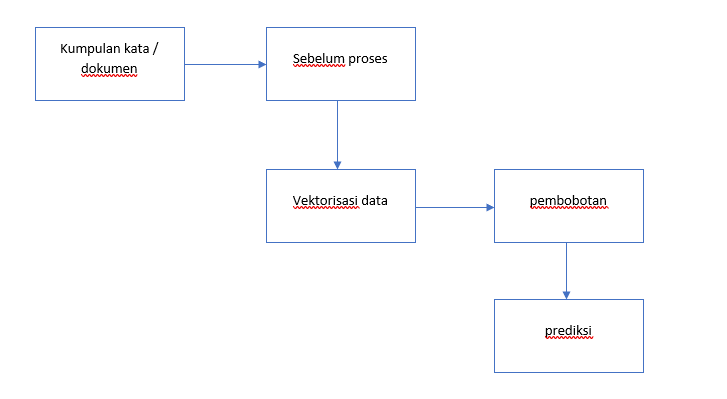
\includegraphics[width=7cm]{figures/1174087/5/1.png}
		\centering
		\caption{Teori 1}
	\end{figure}

	\item Jelaskan mengapa dimensi dari vektor dataset google bisa sampai 300. Dilengkapidengan ilustrasi atau gambar.
	\hfill\break
	Dimensi dataset dari google bisa mencapai 300 karena dimensi dari vektor tersebut digunakan untuk membandingkan bobot dari setiap kata, misalkan terdapat kata dog dan cat pada dataset google tersebut setiap kata tersebut di buat dimensi vektor 300 untuk kata dog dan 300 dimensi vektor juga untuk kata cat kemudian kata tersebt di bandingkan bobot kesamaan katanya maka akan muncul akurasi sekitar 70 persen kesamaan bobot dikarenakan kata dog dan cat sama sama di gunakan untuk hewan priharaan.
	\hfill\break
	\begin{figure}[H]
		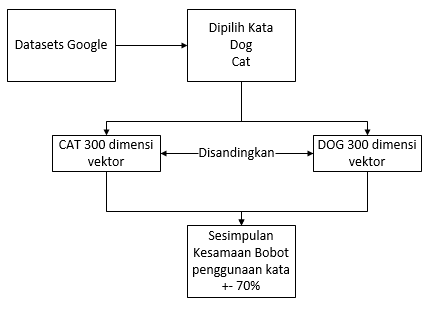
\includegraphics[width=7cm]{figures/1174087/5/2.png}
		\centering
		\caption{Teori 2}
	\end{figure}

	\item Jelaskan konsep vektorisasi untuk kata dilengkapi dengan ilustrasi atau gambar.
	\hfill\break
	Vektorisasi untuk kata untuk mengetahui kata tengah dari suatau kalimat atau kata utama atau objek utama pada suatau kalimat contoh ( Jangan lupa subscribe channel saya ya sekian treimakasih ) kata tengah tersebut merupakan channel yang memiliki bobot sebagai kata tengah dari suatu kalimat atau bobot sebagai objek dari suatu kalimat. hal ini sangat berkaitan dengan dimensi vektor pada dataset google yang 300 tadi karena untuk mendapatkan nilai atau bobot dari kata tengah tersebut di dapatkan dari proses dimensiasi dari kata tersebut. 
	\hfill\break
	\begin{figure}[H]
		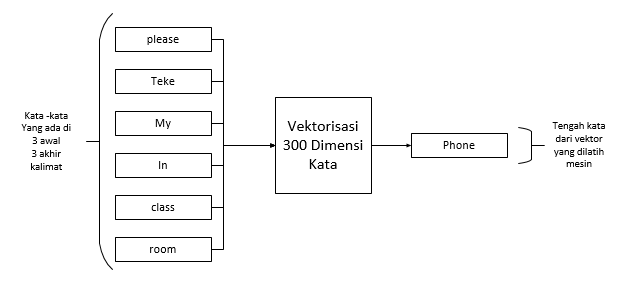
\includegraphics[width=7cm]{figures/1174087/5/3.png}
		\centering
		\caption{Teori 3}
	\end{figure}

	\item Jelaskan konsep vektorisasi untuk dokumen dilengkapi dengan ilustrasi atau gambar.
	\hfill\break
	Vektorisasi untuk dokumen hampir sama seperti vektorisasi untuk kata hanya saja pemilihan kata utama atau kata tengah terdapat pada satu dokumen jadi mesin akan membuat dimensi vektor 300 untuk dokumen dan nanti kata tengahnya akan di sandingkan pada dokumen yany terdapat pada dokumen tersebut.
	\hfill\break
	\begin{figure}[H]
		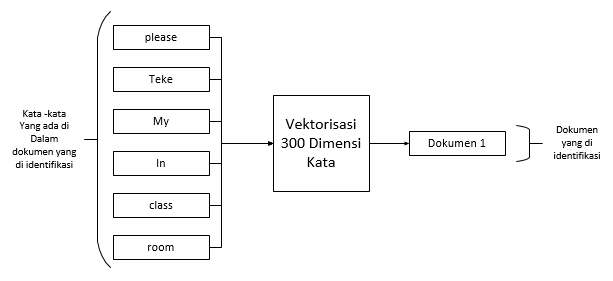
\includegraphics[width=7cm]{figures/1174087/5/4.png}
		\centering
		\caption{Teori 4}
	\end{figure}

	\item Jelaskan apa mean dan standar deviasi,dilengkapi dengan ilustrasi atau gambar.
	\hfill\break
	mean merupakan petunjuk terhadap kata-kata yang di olah jika kata kata itu akurasinya tinggi berarti kata tersebut sering muncul begitu juga sebaliknya, sedangkan setandar defiation merupakan standar untuk menimbang kesalahan. sehingga kesalahan tersebut di anggap wajar misarkan kita memperkirakan kedalaman dari dataset merupakan 2 atau 3 tapi pada kenyataanya merupakan 5 itu merupakan kesalahan tapi masih bisa dianggap wajar karna masih mendekati perkiraan awal.
	\hfill\break
	\begin{figure}[H]
		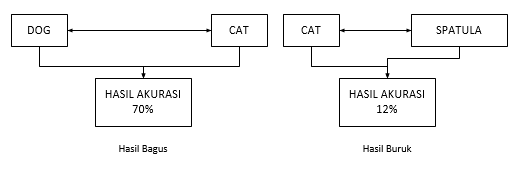
\includegraphics[width=7cm]{figures/1174087/5/5.png}
		\centering
		\caption{Teori 5}
	\end{figure}

	\item Jelaskan apa itu skip-gram,dilengkapi dengan ilustrasi atau gambar.
	\hfill\break
	Skip-Gram adalah kebalikan dari konsep vektorisasi untuk kata dimana kata tengah menjadi acuan terhadap kata kata pelengkap dalam suatu kalimat.
	\hfill\break
	\begin{figure}[H]
		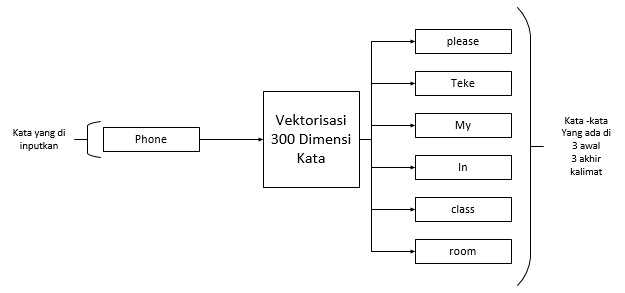
\includegraphics[width=7cm]{figures/1174087/5/6.png}
		\centering
		\caption{Teori 6}
	\end{figure}
\end{enumerate}
\subsection{Praktek}
\begin{enumerate}
	\item Cobalah dataset google, dan jelaskan vektor dari kata love, faith, fall, sick, clear,shine, bag, car, wash, motor, cycle dan cobalah untuk melakukan perbandingan similirati dari masing-masing kata tersebut.
	\begin{itemize}
		\item berikut merupakan code import gensim digunakan untuk membuat data model atau rangcangan data yang akan di buat. selanjutnya dibuat variabel gmodel yang berisi data vektor negativ. selanjutnya data tersebut di load agar data tersebut dapat di tampilkan dan di olah.
		\hfill\break
	\lstinputlisting[firstline=10, lastline=12]{src/1174087/5/1174087.py}	
		\begin{figure}[H]
			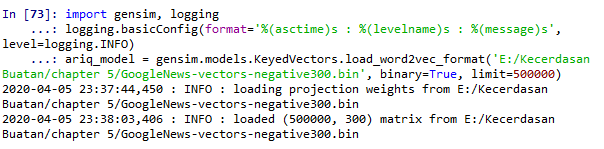
\includegraphics[width=7cm]{figures/1174087/5/7.png}
			\centering
			\caption{Praktek 1}
		\end{figure}
		\item Pada gambar dapat dilihat bahwa vektor love memiliki array sebanyak 300 dimensi. Untuk identitas sektor satu adalah 0.10.
		\hfill\break
		\lstinputlisting[firstline=15, lastline=15]{src/1174087/5/1174087.py}
		\begin{figure}[H]
			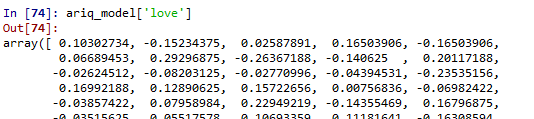
\includegraphics[width=7cm]{figures/1174087/5/8.png}
			\centering
			\caption{Praktek 1.1}
		\end{figure}
		\item Vektor faith dapat dilihat memliki nilai 0.26 , untuk similaritasnya cukup mendekati vektor love dimana faith dapat dikategorikan dalam satu kategori dengan love
		\hfill\break
		\lstinputlisting[firstline=17, lastline=17]{src/1174087/5/1174087.py}
		\begin{figure}[H]
			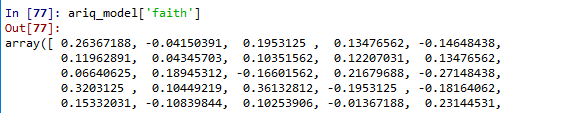
\includegraphics[width=7cm]{figures/1174087/5/9.png}
			\centering
			\caption{Praktek 1.2}
		\end{figure}
		\item Vektor fall hanya memiliki nilai minus yaitu -0.04 , dimana mesin memahami bahwa fall tidak terdapat dalam satu kategori yang sama dengan love dan faith.
		\hfill\break
		\lstinputlisting[firstline=19, lastline=19]{src/1174087/5/1174087.py}
		\begin{figure}[H]
			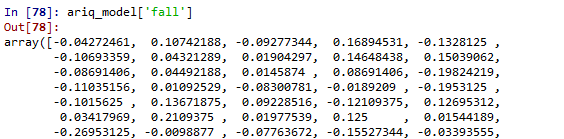
\includegraphics[width=7cm]{figures/1174087/5/10.png}
			\centering
			\caption{Praktek 1.3}
		\end{figure}
		\item Vektor sick memiliki nilai identitas 1.82 dimana tidak mendekati love, faith maupun fall.
		\hfill\break
		\lstinputlisting[firstline=21, lastline=21]{src/1174087/5/1174087.py}
		\begin{figure}[H]
			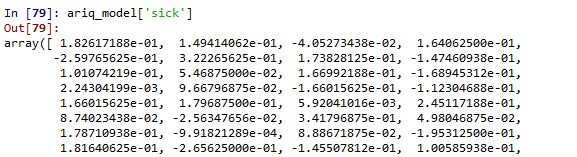
\includegraphics[width=7cm]{figures/1174087/5/11.png}
			\centering
			\caption{Praktek 1.4}
		\end{figure}
		\item Vektor clear memiliki nilai identitas-2,44 dan tidak mendekati nilai dari vektor fall sehingga tidak dapat dijadikan dalam satu kategori.
		\hfill\break
		\lstinputlisting[firstline=23, lastline=23]{src/1174087/5/1174087.py}
		\begin{figure}[H]
			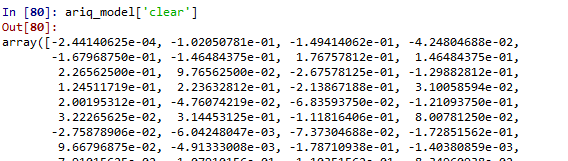
\includegraphics[width=7cm]{figures/1174087/5/12.png}
			\centering
			\caption{Praktek 1.5}
		\end{figure}
		\item Untuk vektor shine -0.12 tidak mendekati vektor manapun. 
		\hfill\break
		\lstinputlisting[firstline=25, lastline=25]{src/1174087/5/1174087.py}
		\begin{figure}[H]
			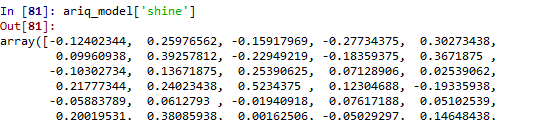
\includegraphics[width=7cm]{figures/1174087/5/13.png}
			\centering
			\caption{Praktek 1.6}
		\end{figure}
		\item Vektor bag memiliki i=nilai identitas -0.03 yang mendekati dengan vektor fall. SEhingga mesin memahami bahwa mungkin saja kedua vektor tersebut berada dalam satu kategori.
		\hfill\break
		\lstinputlisting[firstline=27, lastline=27]{src/1174087/5/1174087.py}
		\begin{figure}[H]
			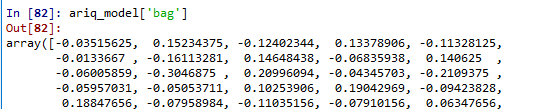
\includegraphics[width=7cm]{figures/1174087/5/14.png}
			\centering
			\caption{Praktek 1.7}
		\end{figure}
		\item Vektor car nilainya 0.13 mendekati vektor love dan faith sehingga mungkin dapat dikategorikan dalam satu kategori.
		\hfill\break
		\lstinputlisting[firstline=29, lastline=29]{src/1174087/5/1174087.py}
		\begin{figure}[H]
			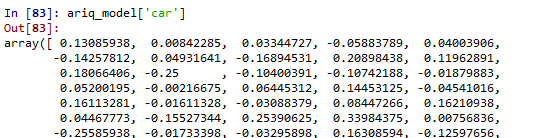
\includegraphics[width=7cm]{figures/1174087/5/15.png}
			\centering
			\caption{Praktek 1.8}
		\end{figure}
		\item Vektor wash memiliki nilai 9.46 jauh dari vektor vektor lainnya.
		\hfill\break
		\lstinputlisting[firstline=31, lastline=31]{src/1174087/5/1174087.py}
		\begin{figure}[H]
			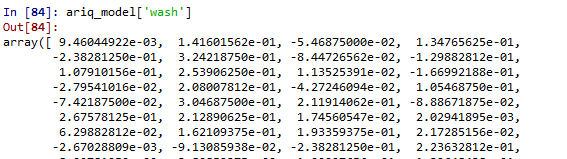
\includegraphics[width=7cm]{figures/1174087/5/16.png}
			\centering
			\caption{Praktek 1.9}
		\end{figure}
		\item Vektor motor memiliki nilai identitas 5.73 yang bisa mendekati vektor wash. Dapat dikatakan bahwa motor dapat dicuci jika diarti dalam satu kategori yang sama.
		\hfill\break
		\lstinputlisting[firstline=33, lastline=33]{src/1174087/5/1174087.py}
		\begin{figure}[H]
			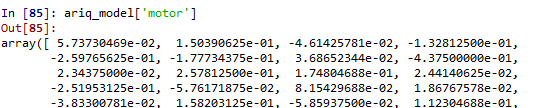
\includegraphics[width=7cm]{figures/1174087/5/17.png}
			\centering
			\caption{Praktek 1.10}
		\end{figure}
		\item Vektor cycle memiliki nilai identitas 0.04
		\hfill\break
		\lstinputlisting[firstline=35, lastline=35]{src/1174087/5/1174087.py}
		\begin{figure}[H]
			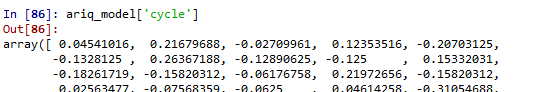
\includegraphics[width=7cm]{figures/1174087/5/18.png}
			\centering
			\caption{Praktek 1.11}
		\end{figure}
		\item berikut merupakan hasil dari similaritas kata kata yang di olah menjadi matrix.
		Dapat disimpulkan bahwa:
		\begin{itemize}
		\item Untuk Love dan faith hasilnya adalah 37 
		\item Untuk Love dan fall hasilnya adalah 11
		\item Untuk Love dan sick hasilnya adalah 26
		\item Untuk Love dan clear hasilnya adalah 6
		\item Untuk Love dan shine hasilnya adalah 20
		\item Untuk Love dan bag hasilnya adalah 7
		\item Untuk Love dan car hasilnya adalah 8
		\item Untuk Love dan wash hasilnya adalah 11
		\item Untuk Love dan motor hasilnya adalah 8
		\item Untuk Love dan wash hasilnya adalah 5
		\end{itemize}
		Artinya love dan faith memang dalam kategori yang sama misalnya dalam kategori percintaan/kepercayaan. Mesin suda hmengetahui bahwa keduanya dapat dikategorikan sebagai percintaan/kepercayaan.

		\hfill\break	
		\lstinputlisting[firstline=37, lastline=55]{src/1174087/5/1174087.py}
		\begin{figure}[H]
			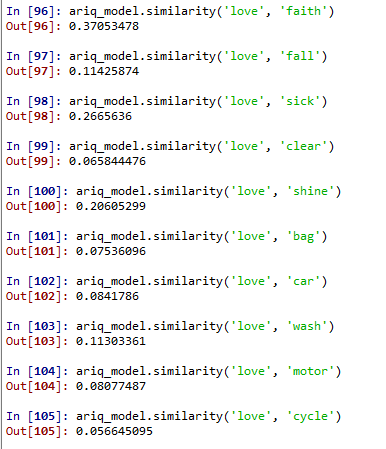
\includegraphics[width=7cm]{figures/1174087/5/19.png}
			\centering
			\caption{Praktek 1.12}
		\end{figure}
	\end{itemize}
	\item Jelaskan dengan kata dan ilustrasi fungsi dari extract words dan PermuteSentences
	\hfill\break
	ExtractWords merupakan function untuk menambahkan, menghilangkan atau menghapuskan, hal hal yang tidak penting atau tidakperlu di dalam teks. Dalam contoh dibawah ini. menggunakan function extract words untuk menghapus komen dengan python style , mencari data yang diinginkan, dan memberikan spasi pada teks.
		\begin{figure}[H]
			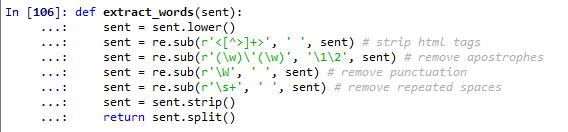
\includegraphics[width=7cm]{figures/1174087/5/20.png}
			\centering
			\caption{Praktek 2}
		\end{figure}
		\hfill\break
		PermuteSentences merupakan class yang digunakan unutm melakukan pengocokan secara acak pada data yang ada. Digunakan cara ini agar tidak terjadi kelebihan memori pada saat dijalankan. 
		\begin{figure}[H]
			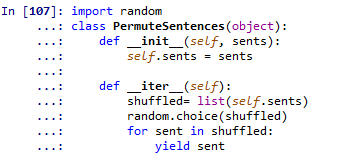
\includegraphics[width=7cm]{figures/1174087/5/21.png}
			\centering
			\caption{Praktek 2}
		\end{figure}

	\item Jelaskan fungsi dari librari gensim TaggedDocument dan Doc2Vec disertai praktek pemakaiannya.
	\hfill\break
	Doc2vec adalah algoritma unsupervised untuk menghasilkan vektor untuk kalimat / paragraf / dokumen. Dan TaggedDocument merupaka function dari Doc2Vec untuk menampilkan tag kata atau kalimat yang diinginkan dari sebuah dokumen.

		\begin{figure}[H]
			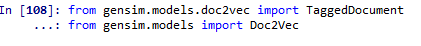
\includegraphics[width=7cm]{figures/1174087/5/22.png}
			\centering
			\caption{Praktek 3}
		\end{figure}
	\item Jelaskan dengan kata dan praktek cara menambahkan data training dari file yang dimasukkan kepada variabel dalam rangka melatih model doc2vac.
	\hfill\break
	
		\begin{figure}[H]
			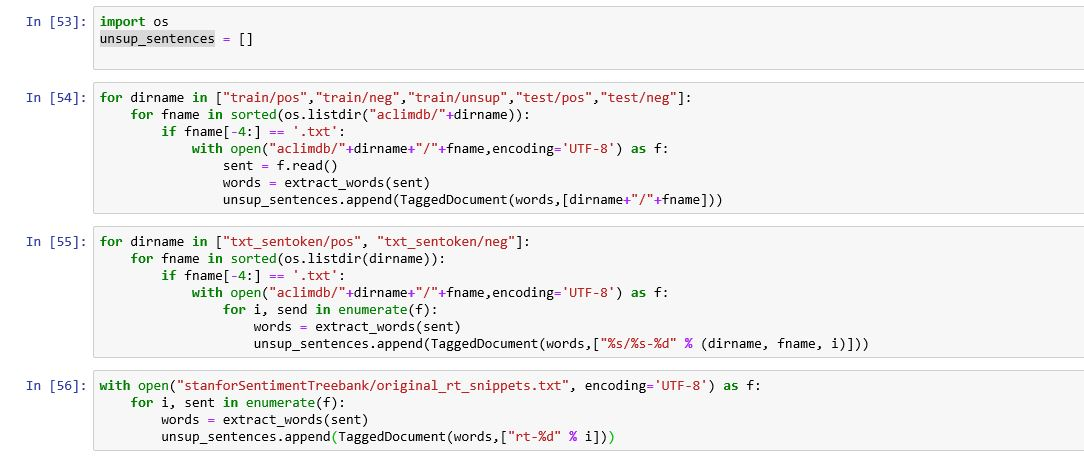
\includegraphics[width=7cm]{figures/1174087/5/23.png}
			\centering
			\caption{Praktek 4}
		\end{figure}
		
	\item Jelaskan dengan kata dan praktek kenapa harus dilakukan pengocokan dan pembersihan data.
	\hfill\break
	Pengocokan dilakukan untuk mendapatkan hasil yang lebih akurat pada saat melakukan score, karena pengocokan mempengaruhi performa positif negatifnya dari scoring. Kemudian Pembersihan data dilakukan untuk membersihkan tag spasi ataupun data noisy yang tidak diperlukan dalam dokumen. 
		\begin{figure}[H]
			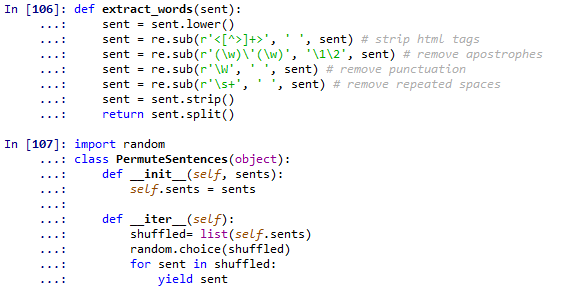
\includegraphics[width=7cm]{figures/1174087/5/24.png}
			\centering
			\caption{Praktek 5}
		\end{figure}
	\item Jelaskan dengan kata dan praktek kenapa model harus di save dan kenapa temporari training harus dihapus.
	\hfill\break
	Model disave untuk memudahkan kita dalam meng-edit file, kita tidak perlu mengetik ulang semua skrip dan tinggal membuka file tersebut jika ingin menguji ulang modelnya. Temporari training merupakan data training yang sebelumnya kita gunakan untuk mencoba skripnya, namun karena kita telah membuat modelnya dan untuk menghemat memori dilakukan penghapusan temporari training agar tidak terjadi lag ataupun hal lainnya.
		\lstinputlisting[firstline=114, lastline=115]{src/1174087/5/1174087.py}
			
	\item Jalankan dengan kata dan praktek maksud dari infer code.
	\hfill\break
	Infer vektor digunakan untuk mengkalkulasikan berapa vektor dari kata yang diberikan. Atau dengan kata lain mengubah kata yang diberikan menjadi bentuk vektor. Dari model yang telah dibuat 
		\begin{figure}[H]
			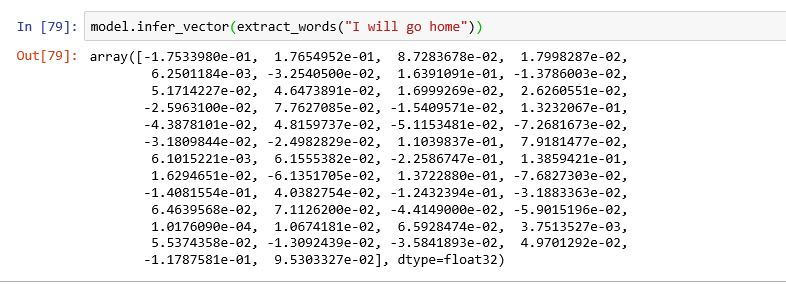
\includegraphics[width=7cm]{figures/1174087/5/26.png}
			\centering
			\caption{Praktek 7}
		\end{figure}

	\item Jelaskan dengan praktek dan kata maksud dari cosine similarity.
	Cosine similarity digunakan untu kmelihat kesamaan atau kemiripan dari suatu kalimat/paragraf yang diinginkan. Apakah kalimat tersebut dapat dikategorikan dalam satu kategori atau tidak.
	\hfill\break
	
		\begin{figure}[H]
			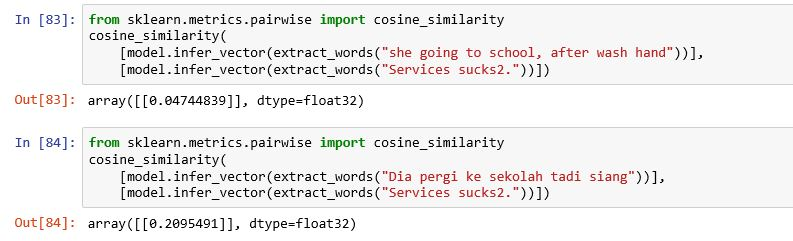
\includegraphics[width=7cm]{figures/1174087/5/27.png}
			\centering
			\caption{Praktek 8}
		\end{figure}
	\item Jelaskan dengan praktek score dari cross validation masing-masing metode.
	\lstinputlisting[firstline=136, lastline=158]{src/1174087/5/1174087.py}	
\end{enumerate}
\subsection{Penangan Error}
\begin{enumerate}
	\item FileNotFound Error
	\hfill\break
		\begin{figure}[H]
			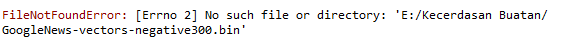
\includegraphics[width=7cm]{figures/1174087/5/error.png}
			\centering
			\caption{FileNotFound Error}
		\end{figure}
	\item Jenis error
	\begin{itemize}
		\item FileNotFound Error
	\end{itemize}
	\item Cara Penanganan
	\hfill\break
	Menyesuaikan tempat/direktori file berada
\end{enumerate}
\subsection{Bukti Tidak Melakukan Plagiat}
\hfill\break
\begin{figure}[H]
	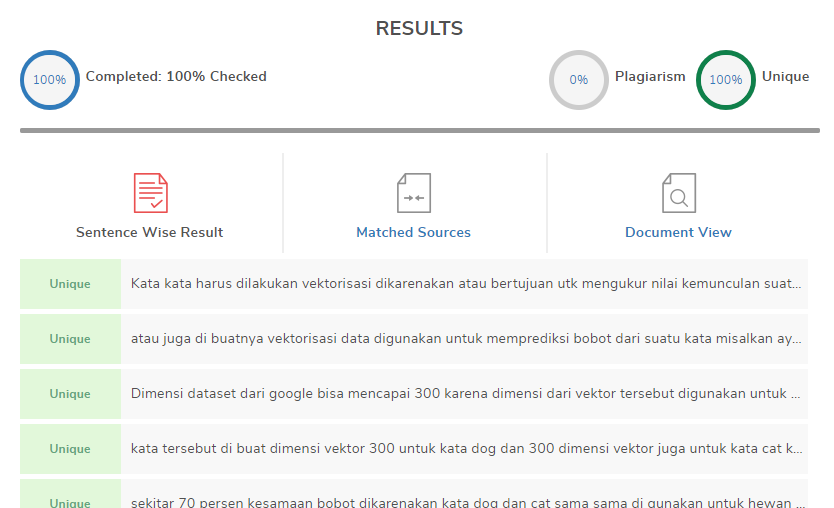
\includegraphics[width=4cm]{figures/1174087/5/plagiat.png}
	\centering
	\caption{Bukti Tidak Melakukan Plagiat}
\end{figure}

\subsection{Link Youtube}
https://youtu.be/vG9L4Ee1KYk